\documentclass[CMPE]{KGCOEReport}
\usepackage{float}
\usepackage{adjustbox}
\graphicspath{ {./images/} }

\newcommand{\name}{Mohammed Fareed \\ Trent Wesley}
\newcommand{\exerciseNumber}{6}
\newcommand{\exerciseDescription}{Motor Control}
\newcommand{\dateDone}{October 18, 2023}
\newcommand{\dateSubmitted}{October 31, 2023}

\newcommand{\classCode}{CMPE 460}
\newcommand{\LabSectionNum}{1}
\newcommand{\LabInstructor}{Prof.\ Hussin Ketout}
\newcommand{\TAs}{Andrew Tevebaugh \\  Colin Vo}
\newcommand{\LectureSectionNum}{1}
\newcommand{\LectureInstructor}{Prof.\ Hussin Ketout}


\begin{document}
\maketitle

\section*{Lab Description}

This laboratory exercise involved interfacing the MSP432 with a DC motor, a stepper motor, and a servo. First, the Timer A module was used to generate a PWM signal. Specifically, a 20\% duty cycle signal with a frequency of 10kHz was generated and viewed with an oscilloscope. Next, a DC motor was controlled. A SN754410 H-bridge IC was utilized to control the 10V power supply voltage with the 3.3V control voltage from the MSP432. The stepper motor was operated in full step, low torque mode by the MSP432 with a ULN2068B Darlington array IC. It was controlled by periodically switching which coils turned on based on the phase. The last type of motor tested was the servo motor. This was controlled by providing a 50Hz PWM signal with a pulse width between 1ms and 2ms. Finally, knowledge gained from testing these motors was used to control the servo and two DC motors on an MSP432-controlled miniature electric car.

\section*{Wiring Diagrams}

\begin{figure}[H]
    \centering
    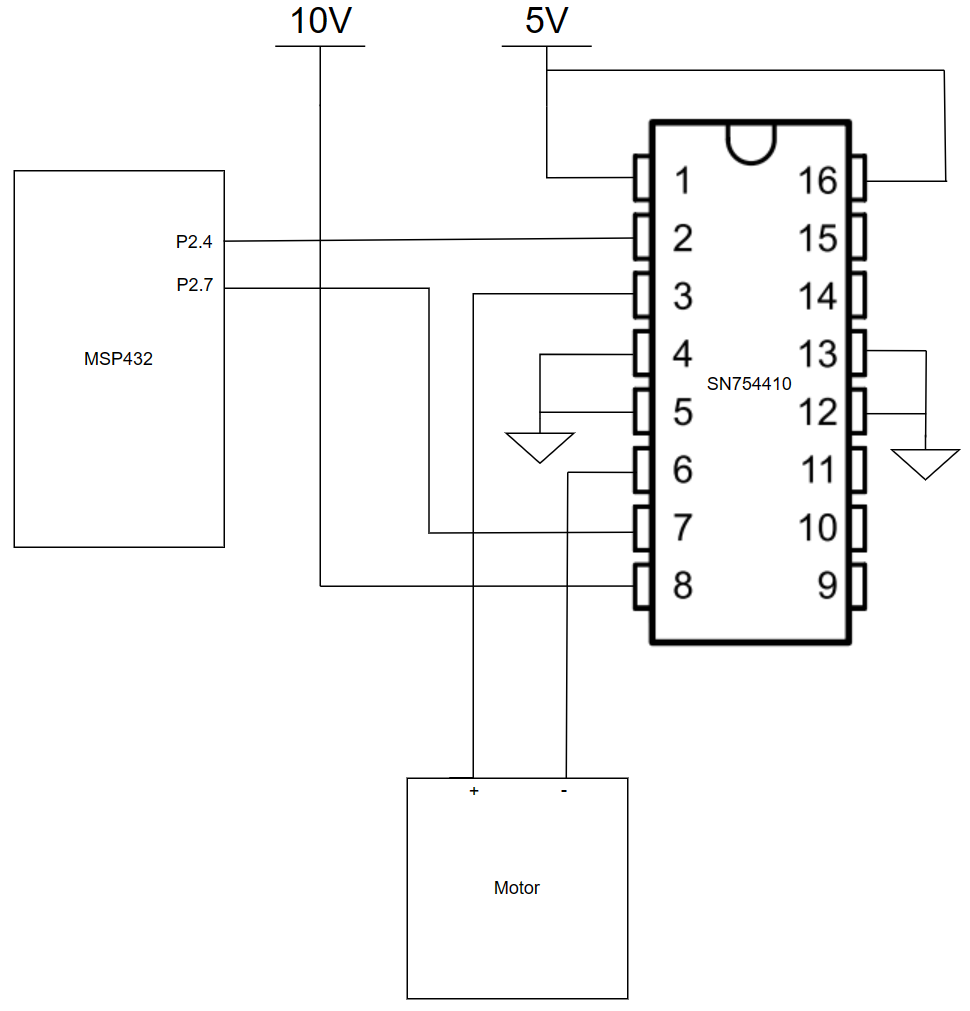
\includegraphics[width=0.75\textwidth]{DCMotorWiring.png}
    \caption{DC Motor Wiring}
    \label{fig:DCMotorWiring}
\end{figure}

\begin{figure}[H]
    \centering
    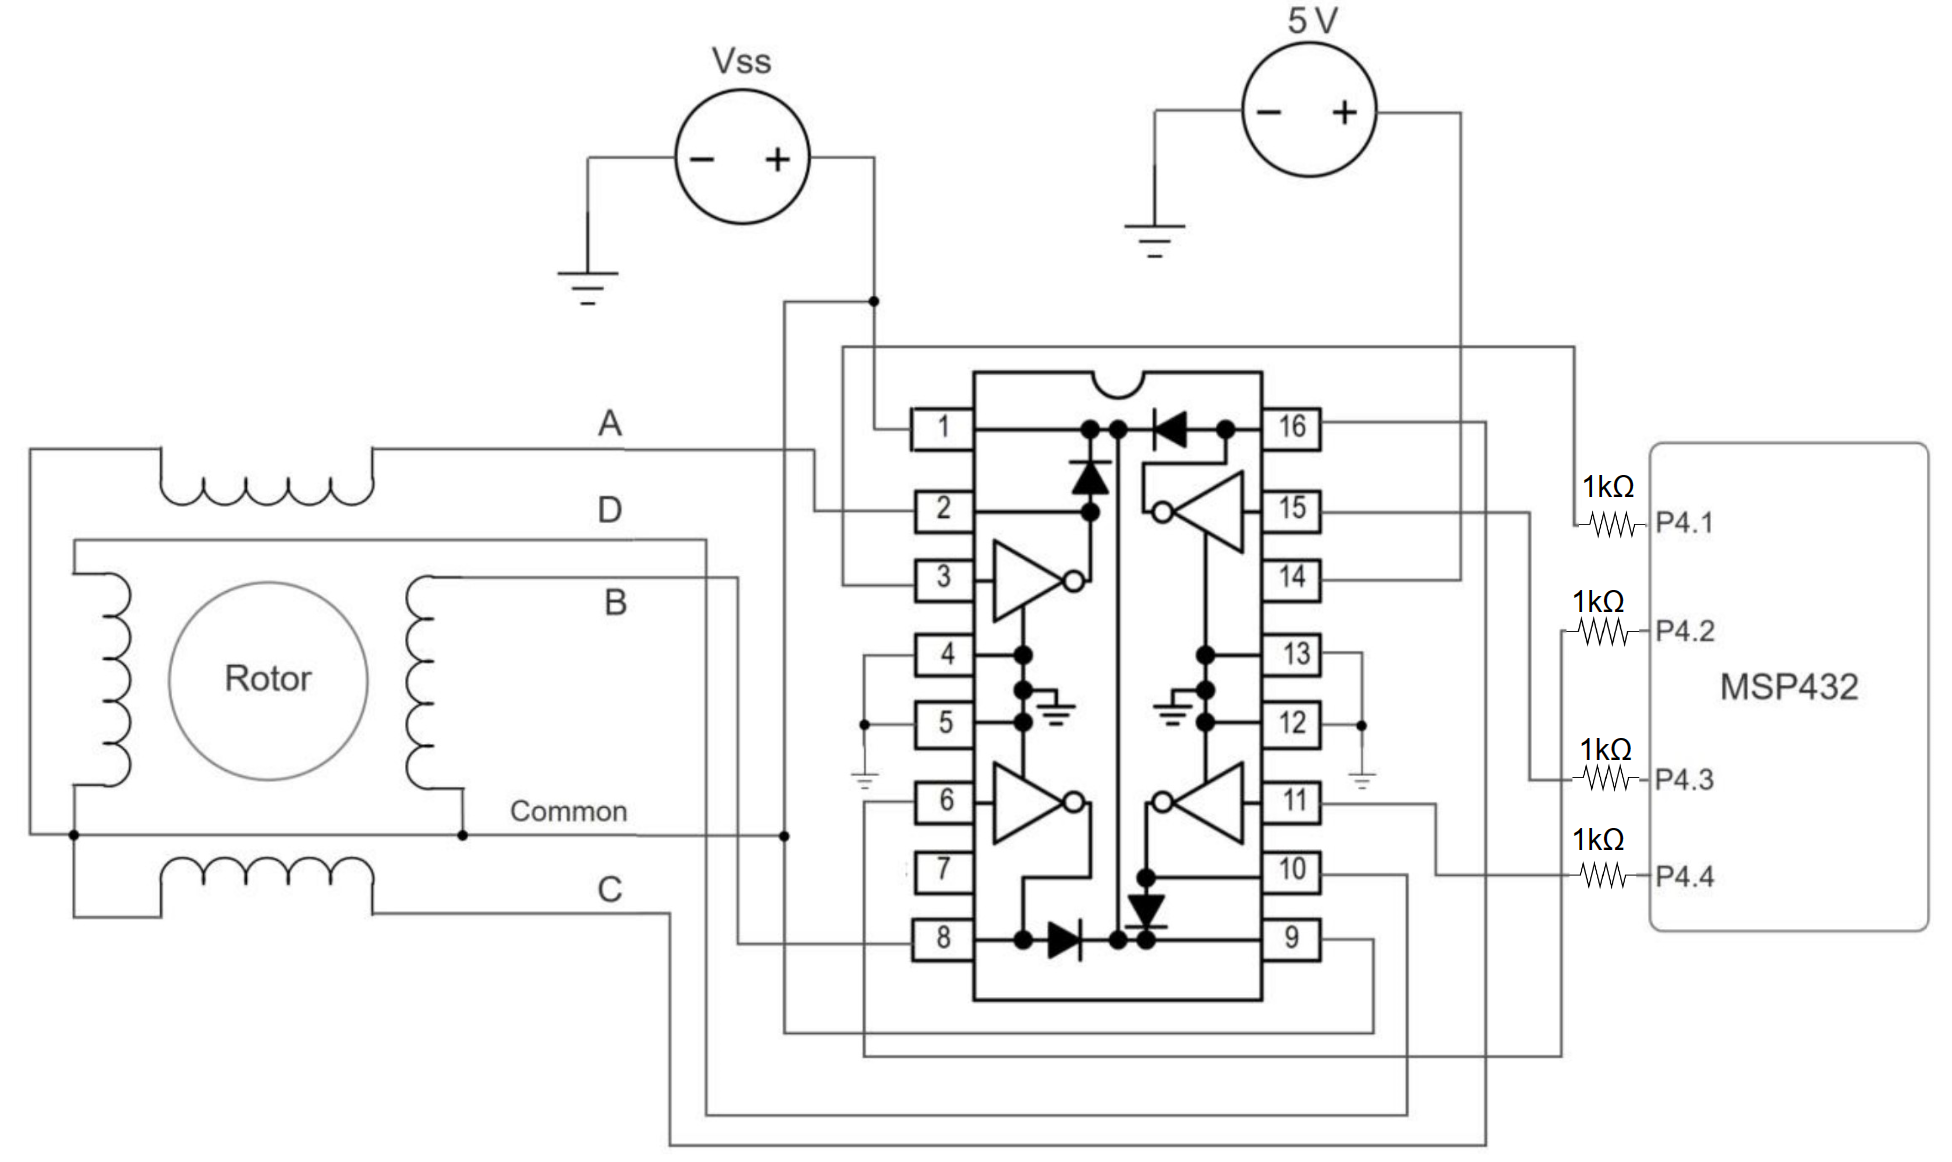
\includegraphics[width=0.75\textwidth]{StepperWiring.png}
    \caption{Stepper Motor Wiring}
    \label{fig:ServoWiring}
\end{figure}

\begin{figure}[H]
    \centering
    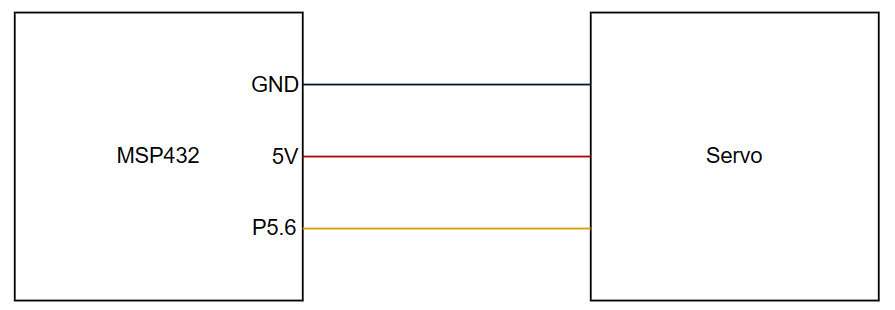
\includegraphics[width=0.75\textwidth]{ServoWiring.png}
    \caption{Servo Wiring}
    \label{fig:SevoWiring}
\end{figure}

\section*{Prelab Questions}

\textbf{Part 1:}\\

\emph{Motor stall torque in oz-in and in kg-cm before reduction}

4.5 kgcm / 30 = 0.15 kgcm = 2.08 oz-in\\

\emph{Maximum current draw}

1.4 A\\

\emph{Maximum motor turn speed before reduction}

0.2 kRPM * 30 = 6 kRPM\\

\emph{Maximum torque in oz-in after gear reduction}

4.5 kgcm = 66.66 oz-in\\

\emph{Maximum turn speed in kRPM after gear reduction}

0.2 kRPM\\

% write in bold Part 2:

\textbf{Part 2:}\\

\emph{What is the purpose of the diodes in this circuit?}

When the motor turns off or changes direction, it can generate a voltage spike due to its inductive nature. These diodes provide a safe path for the induced current to flow, preventing damage to the transistors or other components in the circuit.
\bigskip

\emph{What is the purpose of the capacitor in this circuit?}

The transistor serves decoupling purposes. It can absorb voltage spikes and noise produced by the motor, ensuring that this noise doesn't propagate back into the rest of the circuit or power supply.
\bigskip

\emph{Why are the transistors in each side of the circuit in pairs?}

The pairs form a Darlington pair. This results in a very high current gain, allowing a small input current (from the microcontroller) to control a much larger output current, which can drive the motor.
\bigskip

\emph{Why use 2N3904/2N3906 for some transistors and TIP31/TIP42 for others?}

The 2N3904/2N3906 are general purpose and can only handle low current. The TIP31/TIP42 are power transistors that can handle the high current needed to drive the motor.

\section*{Oscilloscope Captures}

\begin{figure}[H]
    \centering
    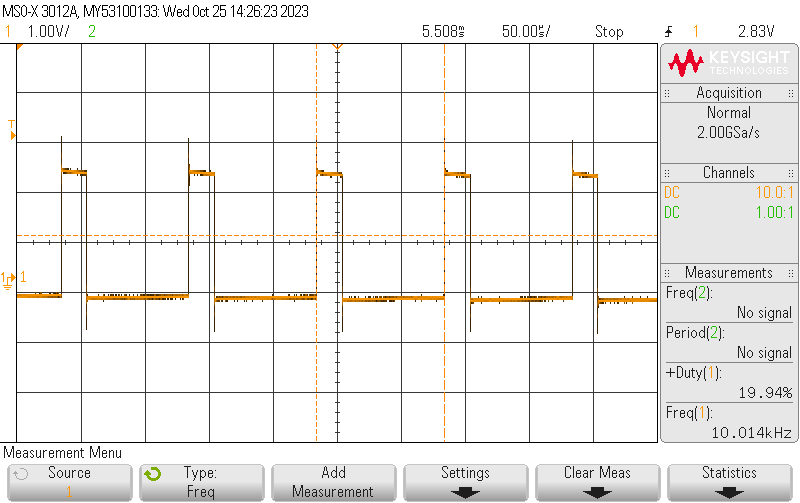
\includegraphics[width=0.75\textwidth]{PWM.png}
    \caption{PWM Waveform}
    \label{fig:pwm}
\end{figure}

\begin{figure}[H]
    \centering
    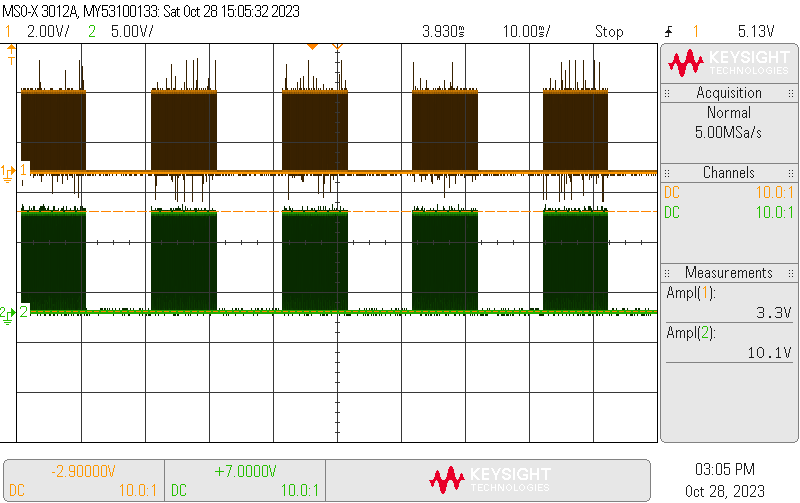
\includegraphics[width=0.75\textwidth]{MotorIO.png}
    \caption{Motor Input Output Waveform}
    \label{fig:motor}
\end{figure}

\begin{figure}[H]
    \centering
    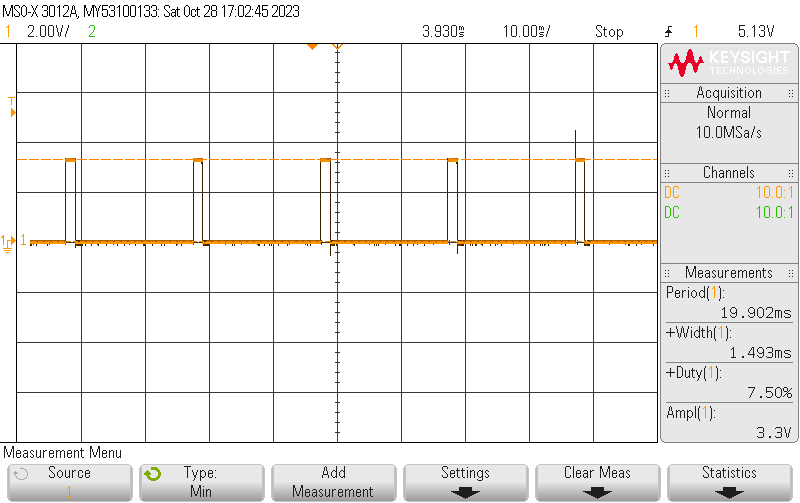
\includegraphics[width=0.75\textwidth]{ServoWave.png}
    \caption{Servo Input Waveform}
    \label{fig:ServoWave}
\end{figure}

\section*{Code Explanation}

Code was written to control a DC motor, a stepper motor, and a servo motor. For the DC motor, the MSP432 was initialized to generate two PWM signals with a 10kHz frequency and a 20\% duty cycle using Timer A0. The code then entered an infinite loop where the duty cycle of the PWM signals was changed to control the speed of the motor. The direction of the motor was changed by switching the PWM and 0V signals to the H-bridge.\\
For the stepper motor, the MSP432 was initialized to output the control signals for the motor's coils using port 4. The code then entered an infinite loop where the coils were turned on and off in a specific order to control the direction of the motor.\\
For the servo motor, the MSP432 was initialized to generate a PWM signal with a 50Hz frequency and a duty cycle between 5\% and 10\%. The code then entered an infinite loop where the pulse width of the PWM signal was changed to control the position of the servo.\\
The DC motors and servo motor code was combined and modified to work with the provided car. The MSP432 was initialized to generate 5 PWM to control 2 DC motors at 10kHz using Timer A0 and one servo motor for steering using Timer A2. The code then entered an infinite loop where the duty cycle of the A0 PWM signals was changed to control the speed of the motors and the A2 pulse width of the PWM signal was changed to control the position of the servo.\\

\section*{Questions}

\emph{Explain how to change speed and direction of turn of the DC motor.}

To change the speed of the DC motor, the duty cycle of the PWM signal from the MSP432 to the H-bridge can be changed. To reverse the direction of the DC motor, the PWM and 0V signals to the H-bridge can be switched.

\bigskip

\emph{Describe an alternate method that uses only one PWM line and one GPIO line.}

An H-bridge can be used to control the direction of the motor. The PWM signal can be used to control the speed of the motor. The GPIO can be used to control the H-bridge to switch which terminal is grounded and which is connected to the PWM line. This allows the GPIO to control the direction, allowing a single PWM to control the speed for both directions.

\bigskip

\emph{Which stepping mode does the code use?}

Full step mode was used.\\

\newpage
\begin{figure}[H]
    \centering
    \begin{adjustbox}{center}
        
\includegraphics[width=1.26\textwidth]{signoff.pdf}
    \end{adjustbox}
\end{figure}

\end{document}
